%!TEX root = francis_thesis.tex
%%%%%%%%%%%%%%%%%%%%%%%%%%%%%%%%%%%%%%%%%%%%%%%%%%%%%%%%%%%%%%%%%%%%%%%
\chapter{Chapter about theory}\label{ch:THEORY}
\section{Computer Vision Tasks}
With the advance of computer vision, task in computer vision has moved from simple tasks  of image classifaication to complex task like semantic and instance segmentation. Deep learning has made this possible, especially using the Vo
\subsection{Image Classification}
Image classification is the process of assigning land cover classes to pixels. Image classification refers to the task of extracting information classes from a multiband raster image. The resulting raster from image classification can be used to create thematic maps. Depending on the interaction between the analyst and the computer during classification, there are two types of classification: supervised and unsupervised. The image classification plays an important role in environmental and socioeconomic applications. In order to improve the classification accuracy, scientists have laid path in developing the advanced classification techniques.
Image classification analyzes the numerical properties of various image features and organizes data into categories. Classification algorithms typically employ two phases of processing: training and testing. In the initial training phase, characteristic properties of typical image features are isolated and, based on these, a unique description of each classification category, i.e. training class, is created. In the subsequent testing phase, these feature-space partitions are used to classify image features. The description of training classes is an extremely important component of the classification process. In supervised classification, statistical processes (i.e. based on an a priori knowledge of probability distribution functions) or distribution-free processes can be used to extract class descriptors. Unsupervised classification relies on clustering algorithms to automatically segment the training data into prototype classes. In either case, the motivating criteria for constructing training classes are that they are:
\begin{enumerate}
\item Independent, e.a change in the description of one training class should not change the value of another,
\item Discriminatory, e.different image features should have significantly different descriptions, and
\item Reliable, all image features within a training group should share the common definitive descriptions of that group.
\end{enumerate}

 This representation allows us to consider each image feature as occupying a point, and each training class as occupying a sub-space (i.e. a representative point surrounded by some spread, or deviation), within the n-dimensional classification space. Viewed as such, the classification problem is that of determining to which sub-space class each feature vector belongs.
\begin{figure}[H]
  \centering
  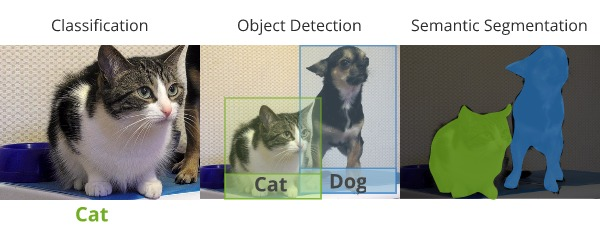
\includegraphics[height=2in]{images/classification_detection_segmentaion_comparisons.jpeg}
   \caption{Image Classification,Object detection Semantic Segmentation.}
\end{figure}
\subsection{Object Detection}
 The goal of object detection is to detect all instances of objects from a known class, such as people, cars or faces in an image. Typically only a small number of instances of the object are present in the image, but there is a very large number of possible locations and scales at which they can occur and that need to somehow be explored.
Each detection is reported with some form of pose information. This could be as simple as the location of the object, a location and scale, or the extent of the object defined in terms of a bounding box. In other situations the pose information is more detailed and contains the parameters of a linear or non-linear transformation. For example a face detector may compute the locations of the
eyes, nose and mouth, in addition to the bounding box of the face. An example of a vehicle and person detection that specifies the locations of certain parts is shown in Figure 1. The pose could also be defined by a three-dimensional transformation specifying the location of the object relative to the camera.
Object detection systems construct a model for an object class from a set of
training examples. In the case of a fixed rigid object only one example may be
needed, but more generally multiple training examples are necessary to capture
certain aspects of class variability.
\begin{figure}[H]
  \centering
  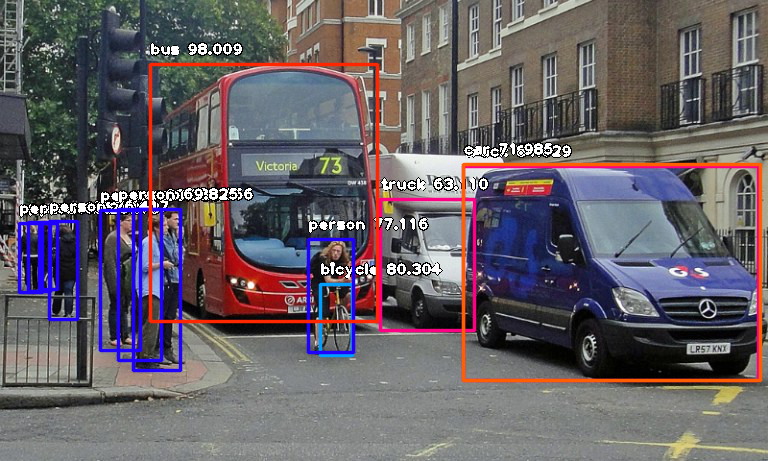
\includegraphics[height=3in]{images/object_det.jpeg}
   \caption{Object detection with bounding boxes.}
\end{figure}

Object detection methods fall into two major categories, generative and discriminative. The first consists of a probability model for the pose variability of the objects together with an appearance model: a probability model for the image appearance conditional on a given pose, together with a model for background, i.e. non-object images. The model parameters can be estimated from training data and the decisions are based on ratios of posterior probabilities. The second typically builds a classifier that can discriminate between images (or sub-images) containing the object and those not containing the object. The parameters of the classifier are selected to minimize mistakes on the training data, often with a regularization bias to avoid overfitting. Other distinctions among detection algorithms have to do with the computational tools used to scan the entire image or search over possible poses, the type of image representation with which the models are constructed, and what type and how much training data is required to build a model.	



\subsection{
Semantic Segmentation
}
Segmentation is essential for image analysis tasks. Semantic segmentation describes the process of associating each pixel of an image with a class label, (such as flower, person, road, sky, ocean, or car).
Semantic image segmentation can be applied effectively to any task that involves the segmentation of visual information. Examples include road segmentation for autonomous vehicles, medical image segmentation, scene segmentation for robot perception, and in image editing tools. Whilst currently available systems provide accurate object recognition, they are unable to delineate the boundaries between objects with the same accuracy.

Oxford researchers have developed a novel neural network component for semantic segmentation that enhances the ability to recognise and delineate objects. This invention can be applied to improve any situation requiring the segmentation of visual information.

Semantic image segmentation plays a crucial role in image understanding, allowing a computer to recognise objects in images. Recognition and delineation of objects is achieved through classification of each pixel in an image. Such processes have a wide range of applications in computer vision, in diverse and growing fields such as vehicle autonomy and medical imaging.

The previous state-of-the-art image segmentation systems used Fully Convolutional Neural Network (FCNN) components, which offer excellent accuracy in recognising objects. Whilst this development represented a significant improvement in semantic segmentation, these networks do not perform well in delineating object boundaries. Conditional Random Fields (CRFs) can be employed in a post-processing step to improve object boundary delineation, however, this is not an optimum solution owing to a lack of integration with the deep network.
\begin{figure}[H]
  \centering
  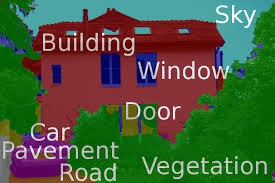
\includegraphics[height=3in]{images/semantic.jpg}
   \caption{Image with semantic segmentation.}
\end{figure}
Oxford researchers have developed a neural network component for semantic segmentation that harnesses the exceptional object recognition of FCNNs and the powerful boundary delineation of CRFs. CRFs are fully integrated as recurrent neural networks, resulting in a system that offers enhanced performance compared to the previous state-of-the-art. The novel system can be applied to any task that involves the segmentation of visual information. Examples include road segmentation for autonomous vehicles, medical image segmentation, scene segmentation for robot perception, and in image editing tools. Oxford University Innovation is seeking industrial partners that wish to explore the use of this system for commercial applications.
\subsection{
Instance Segmentation
}
Instance segmentation is one step ahead of semantic segmentation wherein along with pixel level classification, we expect the computer to classify each instance of a class separately. For example in the image above there are 3 people, technically 3 instances of the class “Person”. All the 3 are classified separately (in a different color). But semantic segmentation does not differentiate between the instances of a particular class.
\begin{figure}[H]
  \centering
  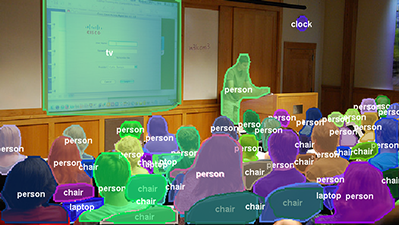
\includegraphics[height=3in]{images/instance.png}
   \caption{Image with instance segmentation.}
\end{figure}

\section{CNN for Object Detection and  Segmentation }

\subsection{Backbone}
\subsubsection{Residual Networks (RESNET)}
ResNet is an essential neural network that serves as a backbone to Mask R-CNN and numerous computer vision tasks. 
It makes the training of extremely deep neural networks possible which was very difficult before then due to the 
challenge of vanishing gradients, that hampers convergence in the network. According to \cite{M} before RESNET, the problem 
of \textit{vanishing gradient} has been mainly addressed by normalized initialization \cite{N},\cite{O}, \cite{P}, \cite{Q} and intermediate 
normalization layers \cite{R}, which enable networks with tens of layers to start converging for stochastic gradient descent 
(SGD) with backpropagation \cite{S}.
Looking at the sample scenario of the vanishing gradients or degradation. A worst-case scenario of vanishing gradient is
 the case was the early layers of a deeper model can be replaced with a shallow network and the other layers can act as an identity function.  The shallow network and its deeper counterpart give the same accuracy. So deeper models do not perform well due to degradation. When a deeper network is used it approximates the mapping than its shallower variant and decreases the error by a notable margin. 
 Also, the deeper network had issues of degradation.
To solve this problem ResNet introduced the concept of skip connection.

\begin{figure}[H]
 \centering
 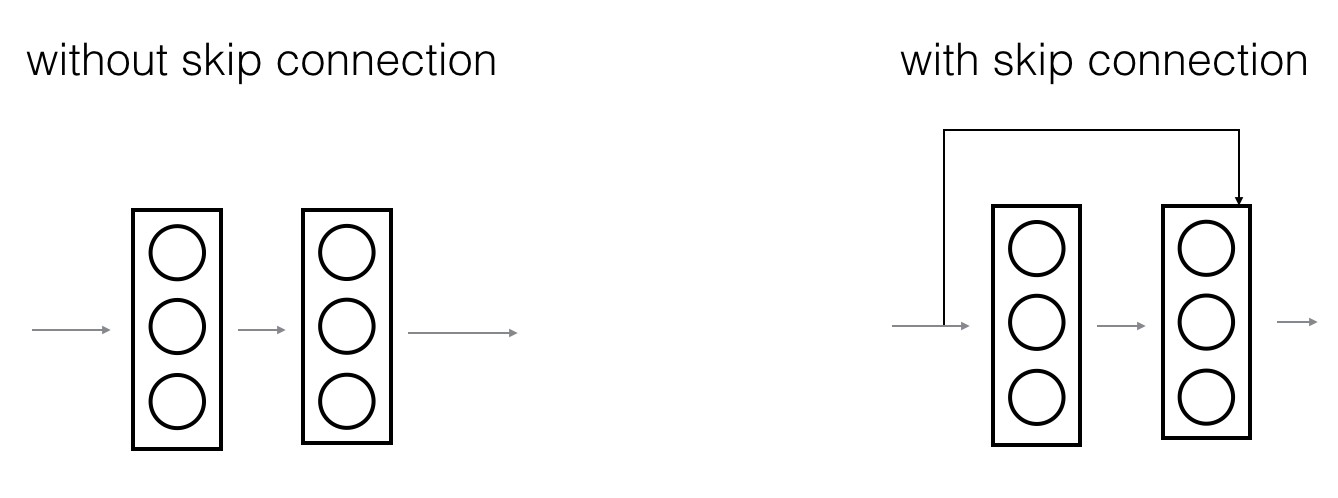
\includegraphics[height=2.3in]{images/skipconnection.jpg}
 \caption{Skip connection of ResNet.}
\end{figure}

Without a skip connection, deep convolution networks are stacked together one after the other.  With a skip connection deep convolution networks are tacked together but this time the original input is added to the output of the convolution block.
Mathematically representing this, we can consider a mapping or space G(x) to be fitted by some stacked layers of an entire network.  X denotes the inputs in the first layer of the net. This layer will approximate a residual function Z(x) = G(x)-x by hypothesizing.  Therefore the original function or mapping G(x) becomes Z(x) + x.  The input and output dimensions are expected to be of the same dimension for this work properly.  It is worth noting that ResNet, contained 152 layers, won ILSVRC 2015 with an error rate of 3.6 percent beating even humans with their error rate of circa 5 – 10 percent, and replacing VGG-16 layers in Faster R-CNN with ResNet-101 produced relative improvements of 28 percent. It also trained networks with 100 layers and 1000 layers. 

\begin{figure}[H]
  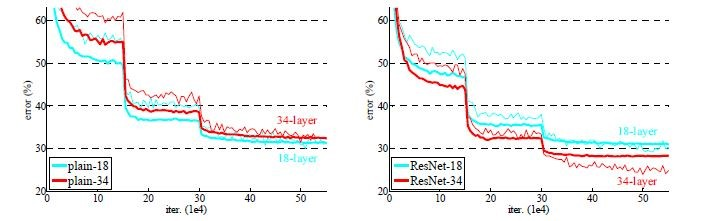
\includegraphics[height=2.2in]{images/resnet-graph.jpg}
   \caption{Training on ImageNet. Thin curves denote training error, and bold curves denote validation error of the center crops. Left: plain networks of 18 and 34 layers. Right: ResNets of 18 and 34 layers. In this plot, the residual networks have no extra parameter compared to their plain counterparts [M].}
\end{figure}

\subsubsection{Feature Pyramid Network}
Feature Pyramid Network (FPN) is a generic feature extractor used in various application for recognizing objects at different scales, developed by Lin et al [K]. For the recognition system for detecting objects at various scales, feature pyramid is a primary constituent of such a system. Pyramid representation has the problem of computing and memory intensiveness and has been avoided in the deep learning object detectors. 
Feature Pyramid Network (FPN) solves this problem by restructuring the architecture of the pyramid to a top-down architecture with lateral connections. The multi-scale, pyramidal hierarchy of deep ConvNet was leveraged to develop Feature Pyramid Network (FPN). Pyramids of  FPN are scale-invariant. This means that when an object scale changes it is offset by shifting its level in the pyramid.  
 Before the introduction of FPN, some ways were used in the extraction of features from images. Initially, hand-engineered features [U] were used and it makes use of featurized image pyramids. ConvNet is more robust to variance in scale, capable of representing higher-level semantics, and so features from it have quickly replaced engineered features. 
 According to \cite{L} this ConvNets gives multi-scale feature representation in which all levels are semantically strong, including the high-resolution levels.  Featuring each level of an image pyramid comes with the profound limitation of increase in inference time which makes it impractical for real applications. FPN explored the pyramidal shape of a ConvNet’s feature hierarchy to build a feature pyramid that has strong features
  with high-resolution at all scales. 
 This gives a feature pyramid that has profound semantics at all phases and is constructed quickly  from a unit  input image scale 
\begin{figure}[H]
\centering
  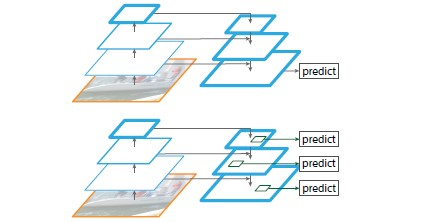
\includegraphics[height=3in]{images/fpn.jpg}
   \caption{Top: a top-down architecture with skip connections, where predictions are made on the finest level (e.g., \cite{T}). Bottom: FPN model that has a similar structure but leverages it as a feature pyramid, with predictions made independently at all levels \cite{K}.}
\end{figure}

FPN was applied in Regional Proposal Network (RPN) and Fast R-CNN. With the new adaptations, RPN could be naturally trained and tested with FPN, Using FPN in a basic Faster R-CNN system, the result surpasses all existing single-model entries including those from the COCO 2016 challenge winners.

\subsection{Regional Proposal Network}
Regional Proposal Network (RPN) is a useful network effectively used in R-CNN that scans the image in a sliding window pattern over the anchors.  It proposes multiple objects that are recognizable in a particular image. The last convolutional layer that is produced by the Faster R-CNN is called the feature map. A proposal is generated for the region where the object lies by sliding over a feature map a network, which is the RPN. RPN suggest where an object lies in an image.
\begin{figure}[H]
\centering
  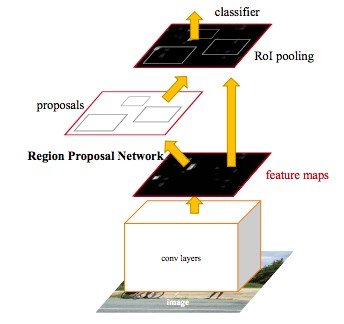
\includegraphics[height=3in]{images/rcnn-rpn.jpg}
   \caption{The architecture of Faster R-CNN. RPN generate the proposal for the objects. \cite{J}.}
\end{figure}

\begin{figure}[H]
\centering
  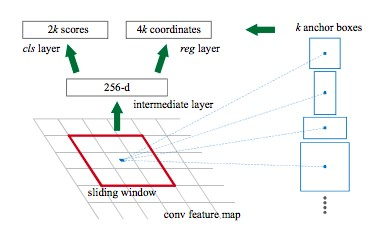
\includegraphics[height=3in]{images/rpn-arch.jpg}
   \caption{RPN Architecture \cite{J}.}
\end{figure}

Analyzing the architecture of RPN, the intermediate layer divides into a classifier and regressor layers, and the 
concept of the anchor was introduced. Anchor are boxes of different sizes and aspect ratio that are generated over an 
image that determines the ideal location, shape, and size of objects in the image. They overlap to fill up as much of 
the image as possible. Thousands of anchor boxes are generated for this. For each anchor box, the object’s bounding box 
that has the highest overlap is divided by non-overlap. This is termed Intersection Over Union (IOU). If the highest IOU 
is greater than 50 percent, the anchor box determines the object that gave the highest IOU. But if it is greater than 40 
percent the true detection is ambiguous, and if it is less than 40 percent it predicts no object. Classifier gives the
 probability of a proposal containing the target object. Regression regresses the coordinates of the proposals. RPN is 
 also used in Mask RCNN.
\begin{figure}[H]
\centering
  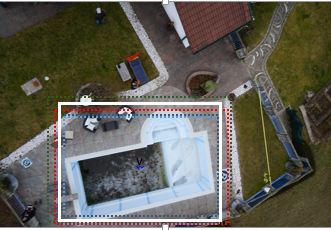
\includegraphics[height=3in]{images/rpn1.png}
   \caption{Anchor boxes (dotted) and the shift/scale applied to them to fit the object precisely (solid). 
   Several anchors can map to the same object.}
\end{figure}

The RPN produces two results for each anchor; Anchor Class i.e. either the foreground or the background, and
 Bounding Box Refinement, an estimation to rectify the anchor box that fits the object well. This is a change in x,y,
  width, height.

\subsection{ROI Classifier and Bounding Box Regressor}
Region of Interest (ROI) classifier is proposed by the Region Proposal Network (RPN) and similarly,
 like the RPN, it produces two results for each ROI. First, the \textit{class}, it produces the classes
  of the object in the ROI, but it is deeper and can classify regions to specific classes (car, person, nucleus, etc). 
  And secondly the\textit{ Bounding Box Refinement}, which further refines the location and size of the bounding box 
  to envelope the object.
\subsubsection{ROI Pooling}
Input sizes of a classifier vary. Classifiers require fixed, stable input size and can’t manage varying input sizes. 
Bounding box refinement in RPN produces ROI boxes of various sizes. ROI Pooling tackles this challenge.
 Cropping a part of a feature map and resizing it to a fixed size is termed ROI pooling. It is very much alike to 
 the concept of resizing a cropped image.
\begin{figure}[H] 
\centering
  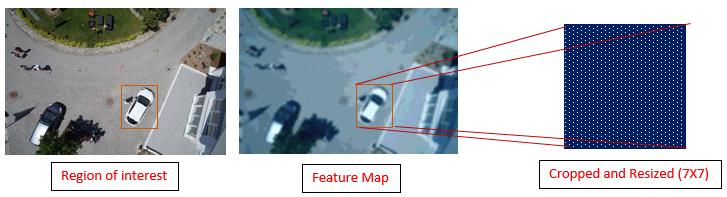
\includegraphics[height=1.8in]{images/roi1.png}
   \caption{ROI Pooling.}
\end{figure}

\subsection{Segmentation Mask}
Mask RCNN further added an extra branch to what Faster RCNN has. This is the mask branch. The Mask branch is a convolutional network that receives the positive regions selected by the ROI classifier and builds low resolution masks for them. The resolution is about 28x 28 pixels. They are soft masks, constituted by float numbers, so they contain more ingredients than binary masks. The size of the mask enables the mask branch to be light. When training the model, the ground-truth masks is scaled down to 28x28 to compute the loss, and when inferencing the predicted masks is scaled up to the size of the ROI bounding box and that produces the final masks, one per object.
\begin{figure}[H]
  \centering
    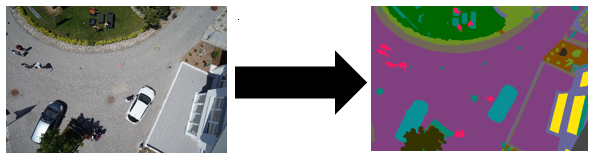
\includegraphics[height=1.7in]{images/mask.png}
     \caption{Segmentation Mask of a drone-based imageset .}
  \end{figure}


\section{Drone-Based Dataset }
Drones (or UAVs) furnished with high resolution cameras have been utilized in a wide range of applications, 
including agricultural, aerial photography, fast delivery, surveillance, etc. This has made, automatic comprehension of 
visual data collected from drones become highly demanding, which brings computer vision to drones more and more closely.
 Outstanding advancements have been made in general computer vision algorithms, such as detection and tracking, yet these algorithms 
 are not usually flawless for dealing with sequences or images captured by drones, due to various difficulties such as view point changes 
 and scales. Consequently, developing and appraising new vision algorithms for drone generated visual data is a key problem in drone-based 
 applications.
The major challenge of segmentation in drone generated visual data is the lack of proper datasets for these. 
A VisDrone Dataset was produced in \cite{V}. The images and video sequences in the benchmark were captured over
 various urban/suburban areas of 14 different cities across China from north to south. Specifically, VisDrone2018 
 consists of 263 video clips and 10; 209 images (no overlap with video clips) with rich annotations, including object 
 bounding boxes, object categories, occlusion, truncation ratios, etc. With intensive amount of effort, our benchmark 
  has more than 2:5 million annotated instances in 179; 264 images/video frames \cite{V}. Also Semantic Drone Dataset that focuses on
   semantic understanding of urban scenes for increasing the safety of autonomous drone flight and landing procedures. The imagery depicts 
   more than 20 houses from nadir (bird's eye) view acquired at an altitude of 5 to 30 meters above ground. A high resolution camera was 
   used to acquire images at a size of 6000x4000px (24Mpx). The training set contains 400 publicly available images and the test set is 
    made up of 200 private images. \cite{W}.

\begin{figure}[H]
  \centering
  
    \includegraphics[height=2.2in]{images/045.jpg}
    \caption{Drone-based imageset 1}
    \label{image 1}
  \end{figure}
  %
  
  \begin{figure}[H]
    \centering
    \includegraphics[height=2.2in]{images/044.jpg}
    \caption{Drone-based imageset 2}
    \label{image 2}
\end{figure}